%
% Artigo Completo para RBIE
%

\documentclass[english, spanish, brazilian]{modelo_dt}
\usepackage[utf8]{inputenc}
\usepackage[T1]{fontenc}
\usepackage{amsmath}
\usepackage{amsfonts}
\usepackage{amssymb}
\usepackage{colortbl}
\definecolor{gray}{gray}{.8}

% Citations and references - Simple approach without biblatex
% \usepackage{mermaid}  % Comentado temporariamente - pacote não disponível

\title{Modelo de Gêmeo Digital Híbrido para Avaliação Multidimensional em Project-Based Learning: Uma Abordagem Integrada de Processos e Sistemas}

\titleinenglish{Hybrid Digital Twin Model for Multidimensional Assessment in Project-Based Learning: An Integrated Process and System Approach}

\titleinspanish{Modelo de Gemelo Digital Híbrido para Evaluación Multidimensional en Aprendizaje Basado en Proyectos: Un Enfoque Integrado de Procesos y Sistemas}

\author{%
	Afonso Cesar Lelis Brandão\\
	Instituto de Tecnologia e Liderança (Inteli)\\
	ORCID: \href{https://orcid.org/0009-0009-4814-9502}{0009-0009-4814-9502}\@.\\
	afonso.brandao@prof.inteli.edu.br\\
	\\
	Reginaldo Arakaki\\
	Instituto de Tecnologia e Liderança (Inteli)\\
	ORCID: \href{https://orcid.org/0000-0003-4718-3425}{0000-0003-4718-3425}\@.\\
	reginaldo.arakaki@prof.inteli.edu.br
}

\Submission{24/Jun/2025}
\First_round_notif{}
\New_version{}
\Second_round_notif{}
\Camera_ready{}
\Edition_review{}
\Available_online{}
\Published{}

\heading{Brandão, A. C. L.; Arakaki, R.}{RBIE v.33 -- 2025}

\citeas{Brandão, A. C. L.; Arakaki, R. (2025). Modelo de Gêmeo Digital Híbrido para Avaliação Multidimensional em Project-Based Learning: Uma Abordagem Integrada de Processos e Sistemas. Revista Brasileira de Informática na Educação, 33, 1--17. https://doi.org/10.5753/rbie.2025.3301}

\begin{document}
\maketitle

\begin{otherlanguage}{brazilian}
\renewcommand{\abstractname}{Resumo}
\begin{abstract}
A avaliação em Project-Based Learning (PBL) apresenta desafios para instituições de ensino superior, particularmente na área de engenharia de software, onde os processos de aprendizagem são multidimensionais e requerem acompanhamento contínuo\@. Este artigo propõe um modelo de gêmeo digital híbrido que integra gêmeos de processo e de sistema para monitoramento e avaliação em tempo real de projetos PBL\@. O modelo baseia-se em três visões arquiteturais -- estrutural, comportamental e de processo -- permitindo análise multidimensional dos domínios pedagógicos, técnicos e de gestão\@. A abordagem coleta dados de repositórios de versionamento, sistemas de gerenciamento educacional, interações orientador-estudante e documentos de projeto, aplicando algoritmos de processamento de linguagem natural e mineração de dados educacionais para extrair insights sobre o progresso da aprendizagem\@. A validação através de case study demonstrou capacidade de identificação precoce de dificuldades de aprendizagem, redução da subjetividade na avaliação e melhoria na qualidade do feedback pedagógico quando comparado aos métodos de avaliação pontual\@.
\keywords{Gêmeos Digitais; Project-Based Learning; Avaliação Educacional; Engenharia de Software; Mineração de Dados Educacionais.}
\end{abstract}
\end{otherlanguage}

\begin{otherlanguage}{english}
\renewcommand{\abstractname}{Abstract}
\begin{abstract}
Assessment in Project-Based Learning (PBL) presents challenges for higher education institutions, particularly in software engineering, where learning processes are multidimensional and require continuous monitoring\@. This paper proposes a hybrid digital twin model that integrates process and system twins for real-time monitoring and assessment of PBL projects\@. The model is based on three architectural views -- structural, behavioral and process -- enabling multidimensional analysis of pedagogical, technical and management domains\@. The approach collects data from repositories, educational management systems, advisor-student interactions and project documents, applying natural language processing algorithms and educational data mining to extract insights about learning progress\@. Validation through case study demonstrated capability for early identification of learning difficulties, reduction of subjectivity in assessment and improvement in pedagogical feedback quality when compared to punctual assessment methods\@.
\keywords{Digital Twins; Project-Based Learning; Educational Assessment; Software Engineering; Educational Data Mining.}
\end{abstract}
\end{otherlanguage}

\begin{otherlanguage}{spanish}
\renewcommand{\abstractname}{Resumen}
\begin{abstract}
La evaluación en Aprendizaje Basado en Proyectos (ABP) presenta desafíos para las instituciones de educación superior, particularmente en ingeniería de software, donde los procesos de aprendizaje son multidimensionales y requieren seguimiento continuo\@. Este artículo propone un modelo de gemelo digital híbrido que integra gemelos de proceso y sistema para monitoreo y evaluación en tiempo real de proyectos ABP\@. El modelo se basa en tres vistas arquitectónicas -- estructural, conductual y de proceso -- permitiendo análisis multidimensional de los dominios pedagógicos, técnicos y de gestión\@. El enfoque recopila datos de repositorios, sistemas de gestión educativa, interacciones asesor-estudiante y documentos de proyecto, aplicando algoritmos de procesamiento de lenguaje natural y minería de datos educativos para extraer insights sobre el progreso del aprendizaje\@.
\keywords{Gemelos Digitales; Aprendizaje Basado en Proyectos; Evaluación Educativa; Ingeniería de Software; Minería de Datos Educativos.}
\end{abstract}
\end{otherlanguage}

\pagebreak

\section{Introdução}

A Aprendizagem Baseada em Projetos (PBL) consolidou-se como uma abordagem educacional ativa, promovendo o desenvolvimento de competências por meio da integração entre teoria e prática, resolução de problemas reais e trabalho colaborativo~(Zhang et al., 2023; Khuankrue & Wongwanich, 2017). Sua adoção em áreas como ciências, saúde, tecnologia e, especialmente, engenharia, reflete o potencial do PBL em aproximar o processo formativo das demandas do mundo profissional.

Apesar de seus benefícios, o PBL impõe desafios significativos à avaliação dos processos de aprendizagem. Em especial na engenharia de software, os projetos desenvolvem-se de forma iterativa e colaborativa, exigindo acompanhamento contínuo para captar a evolução das competências técnicas e transversais dos estudantes~(Kumar & Hsiao, 2022). Os métodos tradicionais de avaliação, centrados em produtos finais e verificações pontuais, mostram-se insuficientes para revelar a complexidade e a dinamicidade do aprendizado experiencial, dificultando a identificação precoce de dificuldades e a oferta de feedback oportuno.

Nesse contexto, cresce a demanda por abordagens avaliativas capazes de acompanhar, em tempo real, o desenvolvimento dos estudantes em múltiplas dimensões. É nesse cenário que os Gêmeos Digitais despontam como uma solução promissora. Originalmente concebidos para simulação e modelagem de sistemas industriais, os gêmeos digitais evoluíram para representar virtualmente entidades reais, mantendo sincronização contínua e possibilitando monitoramento, análise preditiva e otimização de processos (Grieves, 2014; Tao et al., 2018; Barricelli et al., 2019). Suas aplicações na educação têm demonstrado potencial para ampliar o engajamento estudantil e otimizar recursos, ao mesmo tempo em que oferecem novas possibilidades para avaliação formativa~(Zacher, 2020).

A convergência entre as demandas do PBL e as capacidades dos gêmeos digitais sugere uma oportunidade única para transformar a avaliação em ambientes educacionais ativos. Ao permitir o acompanhamento contínuo e a análise multidimensional dos processos de aprendizagem, os gêmeos digitais podem superar as limitações dos métodos tradicionais, fornecendo aos educadores e estudantes informações mais precisas e acionáveis sobre o progresso e as necessidades de desenvolvimento.

Diante desse cenário, este artigo propõe um modelo de gêmeo digital híbrido, integrando perspectivas de processo e sistema, para avaliação multidimensional em projetos PBL de engenharia de software. A proposta fundamenta-se em três visões arquiteturais — estrutural, comportamental e de processo — e utiliza técnicas avançadas de processamento de linguagem natural e mineração de dados educacionais para extrair insights sobre o progresso da aprendizagem, promovendo uma abordagem holística e integrada para avaliação em contextos educacionais dinâmicos.

A convergência entre PBL e tecnologia de gêmeos digitais representa uma oportunidade para a educação em engenharia, particularmente na área de software\@. O modelo proposto neste artigo enquadra-se em uma categoria híbrida que combina características de gêmeo de processo e gêmeo de sistema\@. Esta classificação justifica-se pela natureza do sistema proposto, que visa modelar tanto os processos de aprendizagem quanto os sistemas que suportam esses processos, baseando-se no modelo pedagógico consolidado do Inteli~(Valente & Silva, 2025)@.

\section{Fundamentação Teórica}

\subsection{Project-Based Learning na Educação em Engenharia}

A Aprendizagem Baseada em Projetos (Project-Based Learning — PBL) é uma abordagem pedagógica centrada no estudante, que se consolidou ao longo das últimas décadas como uma das principais metodologias ativas de ensino (Khuankrue & Wongwanich, 2017; Savery, 2015). Suas raízes remontam às ideias do educador John Dewey, no início do século XX, que defendia a aprendizagem por meio da experiência e da resolução de problemas reais, em oposição ao ensino tradicional baseado na transmissão passiva de conteúdos.

O PBL propõe que o processo de aprendizagem seja estruturado em torno de projetos complexos e autênticos, nos quais os estudantes assumam papel ativo na construção do conhecimento. Esses projetos geralmente envolvem a investigação de questões relevantes, a aplicação de conceitos teóricos à prática, o trabalho colaborativo e a produção de artefatos concretos, como relatórios, protótipos ou apresentações {khuankrue2017agent, kolb1984experiential}. O ciclo de aprendizagem experiencial de Kolb, composto por experiência concreta, observação reflexiva, conceituação abstrata e experimentação ativa, fundamenta a dinâmica do PBL e contribui para o desenvolvimento de competências cognitivas, sociais e metacognitivas.

Historicamente, o PBL foi inicialmente adotado em áreas como medicina e ciências da saúde, onde a resolução de casos clínicos e problemas reais é parte essencial da formação profissional. Com o tempo, a metodologia expandiu-se para outras áreas, incluindo ciências exatas, tecnologia, engenharia e matemática (STEM), sendo especialmente valorizada em cursos de engenharia devido à sua capacidade de aproximar o ensino das demandas do mercado de trabalho {zhang2023effectiveness, guo2020systematic}. Em engenharia de software, por exemplo, o PBL permite que os estudantes vivenciem todas as etapas do ciclo de desenvolvimento de sistemas, desde a análise de requisitos até a entrega de soluções, promovendo o desenvolvimento de competências técnicas e transversais essenciais para a atuação profissional~(Valente & Silva, 2025).

Diversos estudos e meta-análises têm demonstrado a eficácia do PBL em comparação com métodos tradicionais de ensino. Os resultados apontam para melhorias significativas no desempenho acadêmico, no desenvolvimento de habilidades de pensamento crítico, resolução de problemas e colaboração {zhang2023effectiveness, balemen2018effectiveness}. Além disso, o PBL contribui para o aumento do engajamento estudantil, da autonomia e da capacidade de aprendizagem ao longo da vida, características fundamentais para profissionais inseridos em contextos de constante transformação tecnológica.

Apesar de seus benefícios, a implementação do PBL apresenta desafios, especialmente no que diz respeito à avaliação dos processos de aprendizagem. A natureza aberta, colaborativa e multidimensional dos projetos dificulta a aplicação de métodos avaliativos tradicionais, exigindo abordagens inovadoras que considerem tanto o produto final quanto o processo de desenvolvimento e as interações entre os participantes.

A avaliação em PBL envolve múltiplas dimensões que se desenvolvem simultaneamente e de forma interdependente. A dimensão técnica abrange o domínio de conhecimentos específicos da área, a capacidade de aplicação de conceitos teóricos na prática e a qualidade dos artefatos produzidos~(Guo et al., 2020). Em engenharia de software, por exemplo, inclui competências como análise de requisitos, design de arquitetura, implementação de código, testes e documentação. A avaliação tradicional, focada em produtos finais, frequentemente falha em capturar a evolução dessas competências ao longo do processo de desenvolvimento.

A dimensão social e colaborativa representa outro desafio significativo. O PBL promove o desenvolvimento de competências como comunicação efetiva, trabalho em equipe, liderança e resolução de conflitos~(Khuankrue & Wongwanich, 2017). No entanto, avaliar essas competências de forma objetiva e contínua é complexo, pois envolve dinâmicas interpessoais que se desenvolvem ao longo do tempo e podem não ser facilmente observáveis através de métodos pontuais de avaliação. A distribuição de responsabilidades, a qualidade das interações entre membros da equipe e a capacidade de colaboração efetiva são aspectos que requerem monitoramento contínuo para serem adequadamente avaliados.

A dimensão metacognitiva, relacionada à capacidade dos estudantes de refletir sobre seu próprio processo de aprendizagem, planejar estratégias e monitorar seu progresso, também apresenta desafios avaliativos~(Kolb, 1984). O desenvolvimento da autonomia, da capacidade de autoavaliação e da aprendizagem ao longo da vida são objetivos fundamentais do PBL, mas sua avaliação requer métodos que permitam capturar processos internos de reflexão e tomada de decisão.

A dimensão temporal representa outro aspecto crítico. Os projetos PBL desenvolvem-se ao longo de períodos extensos, com fases de planejamento, execução, revisão e refinamento. A avaliação tradicional, baseada em verificações pontuais, pode perder informações importantes sobre a evolução das competências, os momentos de dificuldade e superação, e os padrões de desenvolvimento individual e coletivo~(Kumar & Hsiao, 2022). A identificação precoce de dificuldades de aprendizagem e a oferta de feedback oportuno são essenciais para o sucesso do PBL, mas requerem métodos de avaliação que permitam monitoramento contínuo.

A subjetividade na avaliação representa um desafio adicional. A natureza complexa e multidimensional dos projetos PBL torna difícil estabelecer critérios objetivos e padronizados de avaliação. Diferentes avaliadores podem priorizar diferentes aspectos, levando a inconsistências na avaliação. Além disso, a avaliação de competências transversais, como criatividade, pensamento crítico e inovação, frequentemente envolve julgamentos subjetivos que podem variar entre avaliadores~(Zhang et al., 2023).

A escalabilidade da avaliação também representa um desafio prático. Em turmas grandes ou em contextos onde múltiplos projetos são desenvolvidos simultaneamente, o acompanhamento individualizado e a avaliação contínua tornam-se logisticamente complexos. Os métodos tradicionais de avaliação, baseados em revisão manual de produtos e observação direta, não são sustentáveis em contextos de larga escala, exigindo abordagens automatizadas ou semi-automatizadas que mantenham a qualidade da avaliação.

Esses desafios evidenciam a necessidade de abordagens avaliativas inovadoras que sejam capazes de capturar a complexidade multidimensional do PBL, oferecer feedback contínuo e oportuno, e reduzir a subjetividade na avaliação, mantendo a validade e confiabilidade dos processos avaliativos.

\subsection{Gêmeos Digitais: Conceitos e Aplicações Educacionais}

Os Gêmeos Digitais representam uma evolução dos paradigmas de simulação e modelagem de sistemas\@. Grieves\@~(Grieves, 2014) estabelece a definição como uma representação virtual de um objeto, sistema, processo ou entidade que mantém sincronização contínua com seu equivalente real através de dados em tempo real\@. Esta definição diferencia os gêmeos digitais de simulações estáticas, estabelecendo três componentes: a entidade real, sua representação virtual e a conexão bidirecional de dados que permite sincronização contínua\@.

Tao et al.\@~(Tao et al., 2018) expandem a conceituação integrando aspectos de big data e aprendizado de máquina, propondo uma arquitetura que engloba representação virtual, capacidades preditivas e de otimização\@. Esta evolução posiciona os gêmeos digitais como sistemas capazes de antecipar comportamentos, identificar anomalias e sugerir melhorias operacionais\@.

Barricelli et al.\@~(Barricelli et al., 2019) apresentam uma taxonomia que classifica os gêmeos digitais em quatro categorias: (1) gêmeos de componente, que representam elementos individuais; (2) gêmeos de produto ou ativo, que modelam sistemas; (3) gêmeos de sistema, que abrangem conjuntos de ativos interconectados; e (4) gêmeos de processo, que modelam fluxos de trabalho e procedimentos operacionais\@. Para o contexto educacional de PBL, esta categoria possibilita modelagem e avaliação dos processos de aprendizagem\@.

A aplicação de gêmeos digitais na educação tem demonstrado resultados em múltiplos domínios@. Zacher@~(Zacher, 2020) reporta reduções de 26\% nos custos laboratoriais na Universidade de Darmstadt, enquanto estudos na Universidade de Debrecen demonstram que estudantes treinados com gêmeos digitais superaram grupos de controle em tarefas de robótica@~(Kolivand et al., 2021). Lee et al.@~(Hannula et al., 2022) demonstram melhorias no engajamento estudantil através da gamificação em matemática utilizando gêmeos digitais@. A revisão sistemática de Bachmann et al.~(Bachmann et al., 2024) estabelece um framework para aplicações educacionais de gêmeos digitais, categorizando diferentes tipos de implementações e seus benefícios específicos para o contexto educacional@.

\subsection{Integração de PBL e Gêmeos Digitais: O Modelo Híbrido Proposto}

A convergência entre PBL e tecnologia de gêmeos digitais representa uma oportunidade para a educação em engenharia, particularmente na área de software\@. O modelo proposto neste artigo enquadra-se em uma categoria híbrida que combina características de gêmeo de processo e gêmeo de sistema\@. Esta classificação justifica-se pela natureza do sistema proposto, que visa modelar tanto os processos de aprendizagem quanto os sistemas que suportam esses processos, baseando-se no modelo pedagógico consolidado do Inteli~(Valente & Silva, 2025)@.

O gêmeo híbrido diferencia-se de implementações industriais por incorporar dimensões pedagógicas que refletem a complexidade dos processos educacionais\@. Enquanto gêmeos industriais focam em otimização de eficiência e redução de custos, o modelo educacional deve contemplar objetivos de aprendizagem multidimensionais, incluindo desenvolvimento de competências técnicas, transversais e metacognitivas\@.

A arquitetura do gêmeo digital educacional baseia-se na integração das três visões arquiteturais: estrutural, comportamental e de processo\@. A definição destas visões segue os princípios estabelecidos pela norma ISO/IEC/IEEE 42010:2022, que especifica um framework para descrição de arquitetura baseado em viewpoints e views arquiteturais\@. As três visões oferecem perspectivas para compreensão dos processos de aprendizagem em PBL, abrangendo desde a organização estrutural dos recursos até a dinâmica temporal das atividades educacionais\@.

\section{Metodologia}

Esta pesquisa fundamenta-se nos princípios de Design Science Research aplicado ao desenvolvimento de tecnologias educacionais, caracterizando-se pela criação de um artefato conceitual (modelo de gêmeo digital híbrido) para resolver um problema prático: a avaliação contínua e multidimensional em PBL~(Modrakowski & Wiethe-Körprich, 2024). A abordagem metodológica integra desenvolvimento conceitual e validação teórica, com proposta de implementação futura para validação empírica em contexto real de aprendizagem.

A pesquisa adota Design Science Research como paradigma metodológico, estruturada em cinco etapas: (1) identificação do problema e motivação; (2) definição dos objetivos da solução; (3) projeto e desenvolvimento do artefato; (4) demonstração da aplicabilidade; e (5) avaliação da eficácia. Esta estrutura alinha-se com os objetivos estabelecidos e com as características do problema investigado.

O desenvolvimento do modelo iniciou-se com especificação de requisitos funcionais e não funcionais, baseada na análise das necessidades identificadas na literatura sobre avaliação em PBL e nas capacidades técnicas dos gêmeos digitais aplicados em contextos educacionais. A especificação seguiu os princípios estabelecidos pela norma ISO/IEC/IEEE 42010:2022 para descrição de arquiteturas de sistemas.

A modelagem conceitual do gêmeo digital híbrido foi desenvolvida integrando as três visões arquiteturais\@. A arquitetura contempla aspectos estáticos (visão estrutural) e dinâmicos (visões comportamental e de processo) dos projetos PBL, permitindo monitoramento contínuo e análise multidimensional dos processos de aprendizagem\@.

A validação do modelo foi conduzida através de estudo de caso em disciplinas de engenharia de software que adotam metodologia PBL\@. Os critérios de seleção incluíram: adequação dos projetos para demonstração das capacidades do gêmeo digital, disponibilidade de infraestrutura tecnológica, e acessibilidade para coleta de dados sobre o processo de aprendizagem\@.

\section{Modelo Proposto: Gêmeo Digital Híbrido para PBL}

\subsection{Requisitos de Domínio do Problema}

A caracterização do domínio do problema de avaliação em PBL fundamenta-se nos desafios específicos identificados tanto na literatura quanto na experiência prática do modelo pedagógico do Inteli. Esta seção apresenta os requisitos de domínio que emergem da problemática multidimensional da avaliação em ambientes de aprendizagem baseada em projetos, estabelecendo o contexto conceitual que justifica o desenvolvimento do modelo de gêmeo digital híbrido proposto.

\subsubsection{Problemática da Avaliação Multidimensional em PBL}

O domínio do problema caracteriza-se pela complexidade inerente à avaliação de processos de aprendizagem que se desenvolvem simultaneamente em múltiplas dimensões interdependentes. No contexto específico do PBL aplicado em engenharia de software, esta problemática manifesta-se através de desafios que transcendem as capacidades dos métodos avaliativos tradicionais.

\textbf{Desafio da Temporalidade e Continuidade:} Os projetos PBL desenvolvem-se ao longo de períodos extensos (tipicamente 10 semanas no modelo Inteli), com evolução não-linear das competências e marcos de aprendizagem distribuídos temporalmente. A avaliação tradicional, baseada em verificações pontuais, falha em capturar a dinâmica temporal do desenvolvimento de competências, perdendo informações críticas sobre momentos de dificuldade, superação e consolidação do aprendizado. O domínio requer capacidade de monitoramento contínuo que preserve a granularidade temporal das interações e evolução dos artefatos.

\textbf{Desafio da Multidimensionalidade Pedagógica:} O processo de aprendizagem em PBL abrange simultaneamente dimensões técnicas (desenvolvimento de software, aplicação de metodologias, qualidade de código), colaborativas (dinâmicas de equipe, comunicação, liderança), metacognitivas (capacidade de reflexão, autorregulação, aprendizagem autônoma) e processuais (aderência a metodologias ágeis, gestão de tempo, planejamento). A avaliação deve contemplar estas dimensões de forma integrada, identificando correlações e dependências entre elas, sem reduzi-las a métricas isoladas.

\textbf{Desafio da Subjetividade e Variabilidade Avaliativa:} A natureza aberta e criativa dos projetos PBL introduz alta variabilidade nas soluções desenvolvidas pelos estudantes, dificultando a aplicação de critérios objetivos e padronizados. Diferentes orientadores podem priorizar aspectos distintos na avaliação, levando a inconsistências que comprometem a equidade do processo. O domínio requer mecanismos que reduzam a subjetividade sem comprometer a flexibilidade pedagógica necessária para projetos inovadores.

\textbf{Desafio da Escalabilidade e Sustentabilidade:} O acompanhamento individualizado de múltiplas equipes desenvolvendo projetos complexos representa desafio logístico significativo, especialmente em contextos de larga escala. O modelo tradicional baseado em observação direta e revisão manual torna-se insustentável quando aplicado a dezenas de equipes simultâneas. O domínio necessita de abordagens que mantenham a qualidade da avaliação independentemente da escala de aplicação.

\subsubsection{Especificidades do Contexto Inteli}

O modelo pedagógico do Inteli apresenta características específicas que ampliam a complexidade do domínio do problema:

\textbf{Integração com Parceiros Externos:} Os projetos são desenvolvidos em colaboração com empresas parceiras, introduzindo requisitos reais e expectativas de mercado que devem ser consideradas na avaliação. Esta integração cria tensão entre objetivos de aprendizagem e demandas comerciais, exigindo balanceamento cuidadoso na avaliação de competências versus entrega de valor para o parceiro.

\textbf{Metodologia de Sprints e Entregas Incrementais:} A estrutura em sprints de 2 semanas com entregas incrementais cria múltiplos pontos de avaliação que devem ser integrados em uma visão holística do progresso. Cada sprint representa um ciclo completo de desenvolvimento, mas a avaliação deve considerar a evolução acumulativa ao longo de todos os sprints.

\textbf{Diversidade de Perfis e Backgrounds:} Os estudantes apresentam níveis heterogêneos de experiência prévia em tecnologia e metodologias de desenvolvimento, criando trajetórias de aprendizagem diferenciadas que devem ser consideradas na avaliação. O domínio deve acomodar esta diversidade sem comprometer os padrões de qualidade esperados.

\textbf{Autogestão e Autonomia Estudantil:} O modelo pedagógico promove alta autonomia estudantil na organização do trabalho e tomada de decisões técnicas. Esta autonomia, embora desejável para o desenvolvimento de competências profissionais, complica a avaliação ao reduzir a visibilidade direta dos orientadores sobre os processos internos das equipes.

\subsubsection{Requisitos Emergentes do Domínio}

Desta caracterização da problemática emergem os seguintes requisitos de domínio que devem ser endereçados pelo modelo proposto:

\textbf{Captura Multidimensional Integrada:} O domínio requer capacidade de coletar e correlacionar dados de múltiplas fontes (repositórios de código, ferramentas de comunicação, documentos de projeto, interações orientador-estudante) para construir uma visão integrada do processo de aprendizagem que preserve as interdependências entre dimensões.

\textbf{Análise Temporal Contextualizada:} É necessário processar dados temporais considerando o contexto específico de cada momento do projeto (início de sprint, entregas intermediárias, revisões de código, apresentações para parceiros), identificando padrões e anomalias que indiquem necessidade de intervenção pedagógica.

\textbf{Redução de Subjetividade com Preservação de Flexibilidade:} O domínio demanda mecanismos que objetivem a avaliação através de métricas e evidências quantificáveis, mantendo espaço para julgamento pedagógico qualitativo e consideração de contextos específicos de cada projeto e equipe.

\textbf{Identificação Precoce de Riscos de Aprendizagem:} É essencial detectar precocemente indicadores de dificuldades de aprendizagem, isolamento social, sobrecarga de trabalho ou desalinhamento com objetivos pedagógicos, permitindo intervenções oportunas que previnam comprometimento do processo formativo.

\textbf{Feedback Contextual e Acionável:} O domínio requer geração de feedback personalizado que considere o perfil individual do estudante, o momento específico do projeto e o contexto da equipe, oferecendo orientações concretas para melhoria e recursos de apoio direcionados.

\textbf{Transparência e Explicabilidade:} É fundamental que estudantes e orientadores compreendam os critérios e processos utilizados na avaliação, mantendo a confiança no sistema e possibilitando contestação e refinamento contínuo dos mecanismos avaliativos.

Estes requisitos de domínio estabelecem o contexto conceitual que justifica e direciona o desenvolvimento do modelo de gêmeo digital híbrido, definindo as problemáticas específicas que devem ser endereçadas para criar uma solução efetiva para avaliação multidimensional em ambientes PBL. A arquitetura e funcionalidades propostas nas seções seguintes são concebidas especificamente para atender a estes requisitos emergentes da caracterização detalhada do domínio do problema.

\subsection{Arquitetura Conceitual}

O modelo proposto fundamenta-se na premissa de que os processos de aprendizagem em PBL e os sistemas que os suportam podem ser modelados e monitorados através de um gêmeo digital híbrido que mantém sincronização contínua com as atividades educacionais reais e a infraestrutura tecnológica subjacente\@.

O gêmeo digital híbrido integra duas categorias da taxonomia estabelecida por Barricelli et al.\@~(Barricelli et al., 2019): (1) gêmeo de processo, que modela e monitora o processo de aprendizagem em si, incluindo progressão temporal das competências, dinâmicas de equipe e eficácia das intervenções pedagógicas; e (2) gêmeo de sistema, que representa virtualmente o produto de software desenvolvido pelos estudantes, incluindo arquitetura técnica, qualidade de código e evolução temporal do sistema\@.

\begin{figure}[htbp]
\centering
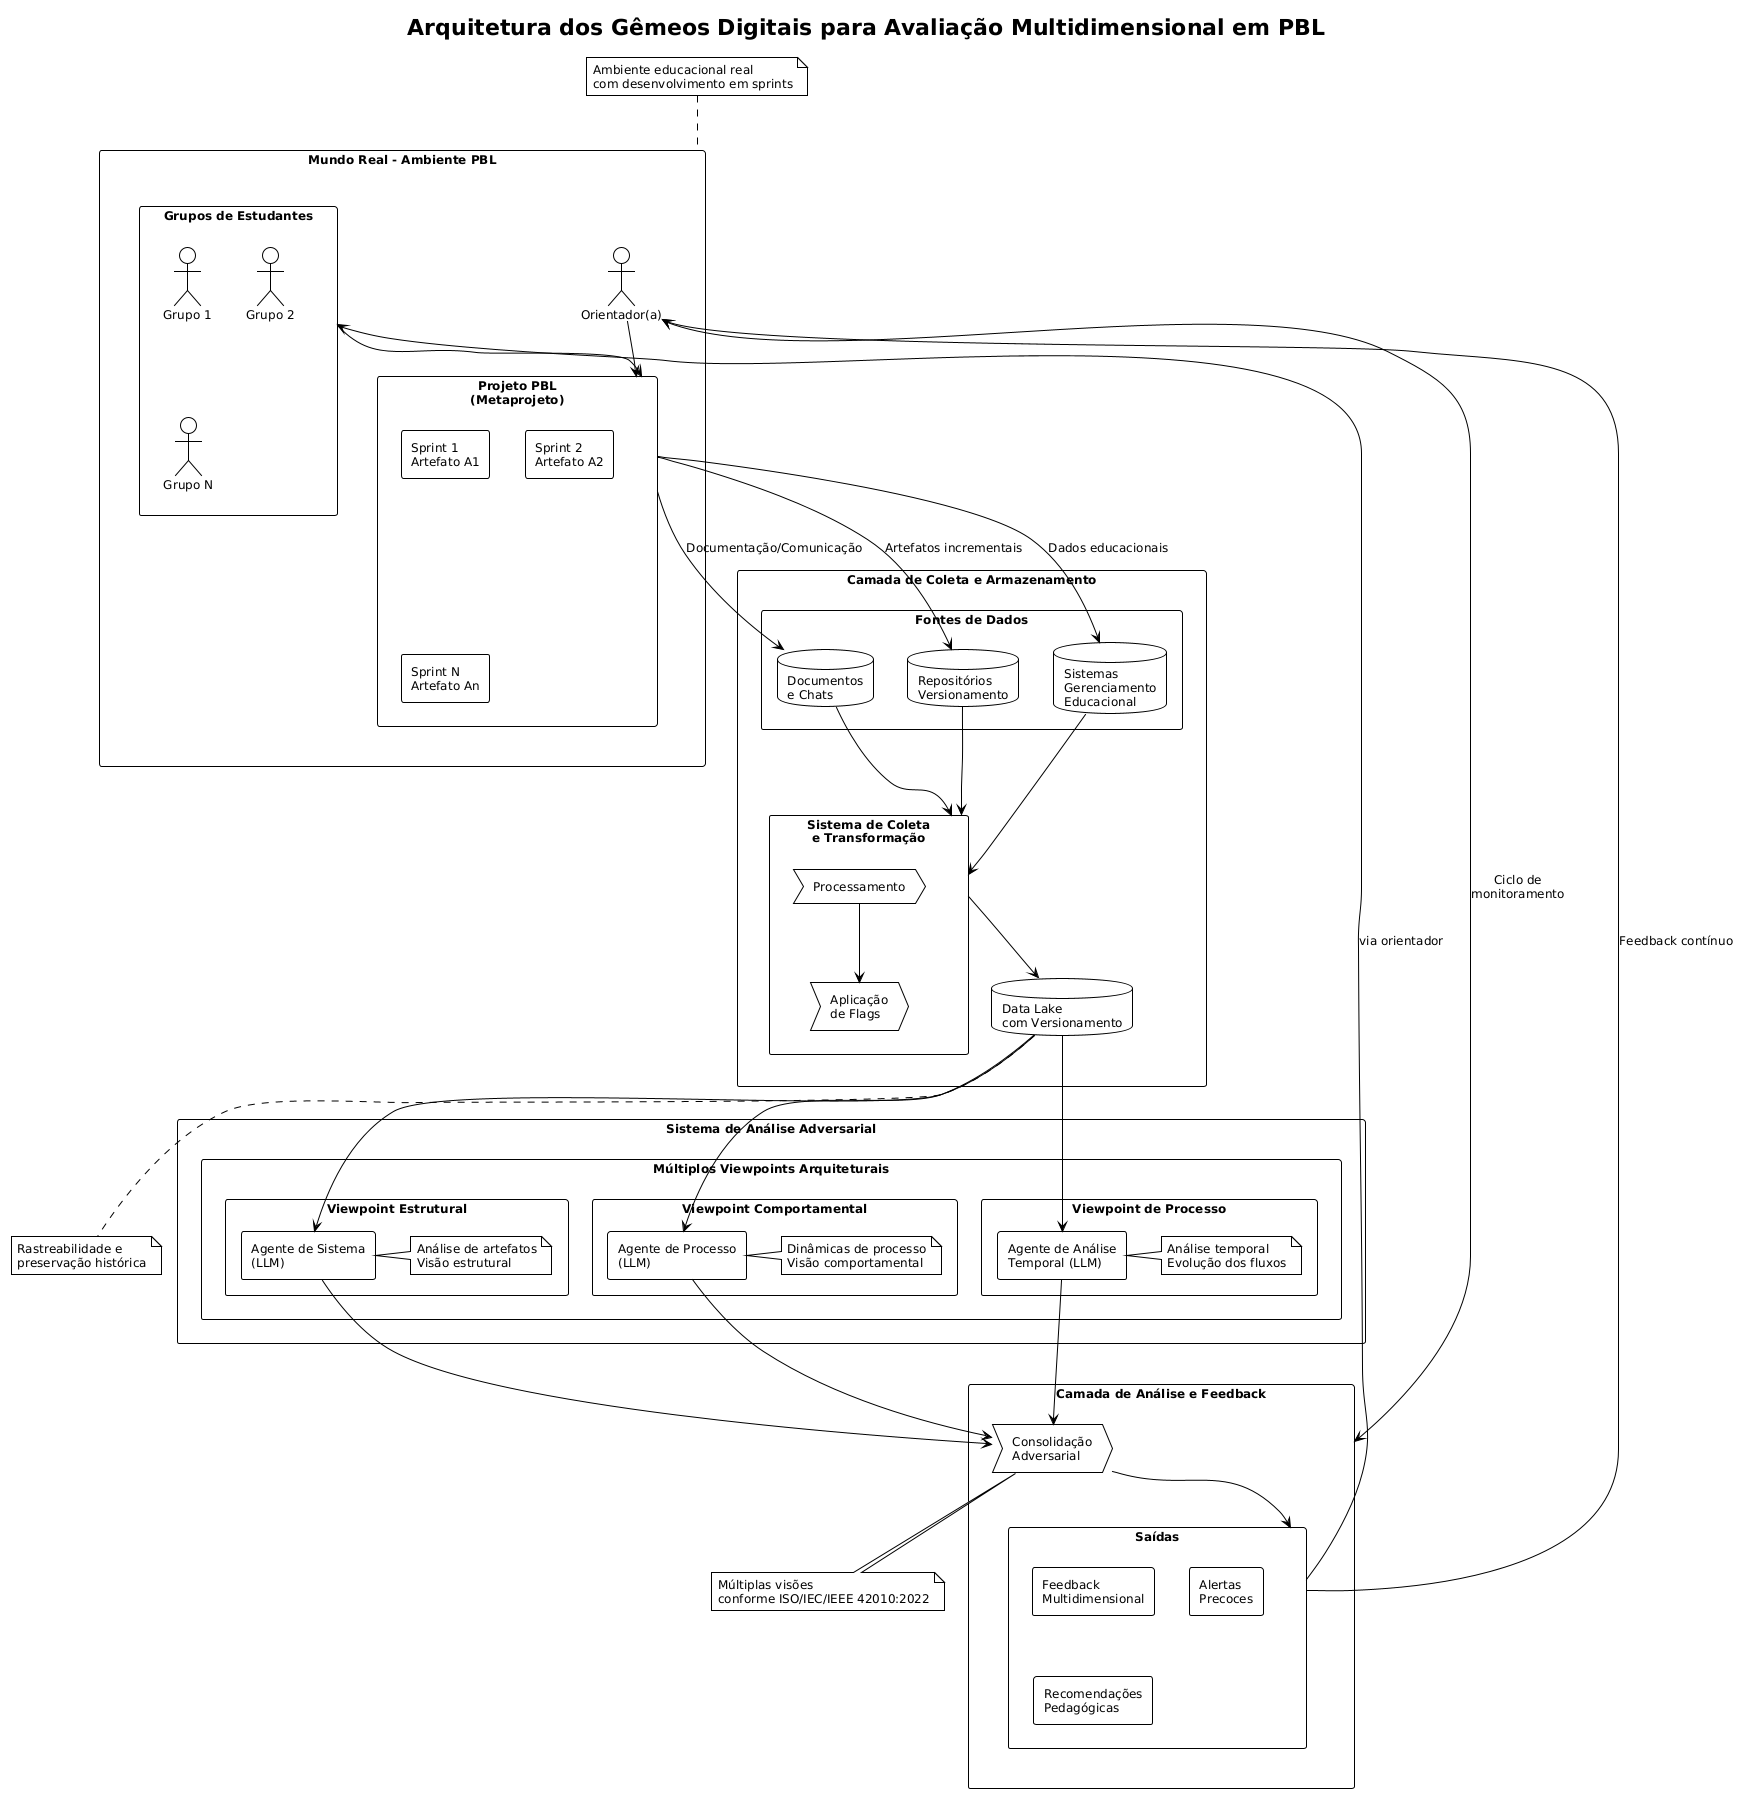
\includegraphics[width=\linewidth,height=0.8\textheight,keepaspectratio]{assets/f1.png}
\caption{Arquitetura dos Gêmeos Digitais para Avaliação Multidimensional em PBL}
\label{fig:gemeo-digital-pbl}
\end{figure}

A Figura~\ref{fig:gemeo-digital-pbl} ilustra a arquitetura completa do gêmeo digital híbrido, mostrando a integração entre o mundo real (PBL Inteli) e sua representação virtual. O modelo estabelece uma conexão bidirecional contínua, permitindo monitoramento em tempo real e feedback imediato para estudantes e orientadores\@.

\textbf{Descrição da Arquitetura:} O gêmeo digital híbrido opera através de uma arquitetura em camadas que conecta o ambiente educacional real ao sistema de análise adversarial. A arquitetura é composta por:

\textbf{(1) Mundo Real - Ambiente PBL:} Inclui o orientador(a), estudantes organizados em grupos, e o projeto PBL (metaprojeto) que estrutura as atividades educacionais. Os projetos são desenvolvidos em sprints iterativos, gerando artefatos incrementais (A1, A2, ..., An) que representam marcos de aprendizagem e desenvolvimento\@.

\textbf{(2) Camada de Coleta e Armazenamento:} Integra múltiplas fontes de dados (repositórios de versionamento, sistemas de gerenciamento educacional, documentos e chats) através de um sistema de coleta e transformação que realiza processamento e aplicação de flags para categorização. Os dados processados são armazenados em um lago de dados (Data Lake) com versionamento, garantindo rastreabilidade e preservação histórica das informações@.

\textbf{(3) Sistema de Análise Adversarial:} Implementa três viewpoints arquiteturais especializados, cada um operando através de agentes de modelos de linguagem grandes (Large Language Models -- LLM) independentes:
\begin{itemize}
\item \textbf{Viewpoint Estrutural}: Focado na análise de artefatos e visão estrutural dos projetos, operado pelo Agente de Sistema
\item \textbf{Viewpoint Comportamental}: Especializado em dinâmicas de processo e visão comportamental, operado pelo Agente de Processo
\item \textbf{Viewpoint de Processo}: Dedicado à análise temporal e evolução dos fluxos de trabalho
\end{itemize}

\textbf{(4) Camada de Análise e Feedback:} O sistema de análise adversarial com agentes LLM processa os dados dos três viewpoints, gerando feedback multidimensional, alertas precoces e recomendações pedagógicas que retornam ao orientador(a) e, consequentemente, aos estudantes e grupos\@.

O fluxo de dados é bidirecional e contínuo: os artefatos gerados em cada sprint alimentam as fontes de dados, que são processadas e armazenadas no Data Lake. Os agentes LLM dos diferentes viewpoints acessam esses dados para realizar análises especializadas, que são consolidadas no sistema adversarial para gerar insights e feedback que retornam ao ambiente educacional, fechando o ciclo de monitoramento e intervenção pedagógica\@.

\subsection{Visões Arquiteturais Integradas}

Conforme estabelecido pela norma ISO/IEC/IEEE 42010:2022, o modelo implementa três viewpoints para capturar diferentes aspectos dos processos de aprendizagem\@.

\subsubsection{Viewpoint Estrutural}

O viewpoint estrutural mapeia a organização estática dos projetos PBL, incluindo estrutura das equipes, distribuição de recursos, arquitetura dos artefatos produzidos e configuração do ambiente de desenvolvimento\@. Esta visão permite identificação de lacunas organizacionais e inadequações na alocação de recursos que possam impactar o desempenho das equipes, facilitando intervenções para otimização da estrutura de suporte ao aprendizado\@.

Os componentes principais desta visão incluem:
\begin{itemize}
\item \textbf{Estrutura das equipes}: Composição, papéis definidos, distribuição de responsabilidades e rotação de funções
\item \textbf{Distribuição de recursos}: Alocação de ferramentas tecnológicas, acesso a laboratórios e recursos bibliográficos
\item \textbf{Arquitetura dos artefatos}: Organização dos deliverables, documentação técnica e produtos intermediários
\item \textbf{Configuração do ambiente}: Setup de desenvolvimento, ferramentas de colaboração e repositórios de código
\end{itemize}

\subsubsection{Viewpoint Comportamental}

O viewpoint comportamental modela as interações dinâmicas entre os participantes do processo educacional, capturando padrões de colaboração, comunicação, dinâmicas de resolução de problemas e desenvolvimento de competências transversais\@. Esta visão revela aspectos do processo de aprendizagem difíceis de capturar através de métodos de avaliação pontuais\@.

Os elementos monitorados incluem:
\begin{itemize}
\item \textbf{Padrões de colaboração}: Frequência e qualidade das interações entre membros da equipe
\item \textbf{Comunicação}: Canais utilizados, efetividade das trocas de informação e clareza na documentação
\item \textbf{Resolução de problemas}: Estratégias adotadas para superação de obstáculos e busca por ajuda externa
\item \textbf{Competências transversais}: Evolução de habilidades de liderança, trabalho em equipe e gestão de tempo
\end{itemize}

\subsubsection{Viewpoint de Processo}

O viewpoint de processo representa os fluxos temporais de atividades, contemplando marcos de entrega, aderência a metodologias, evolução qualitativa e ciclos de desenvolvimento\@. Esta visão oferece visibilidade sobre a qualidade dos processos adotados pelas equipes e sua conformidade com as práticas da engenharia de software\@.

Os aspectos monitorados incluem:
\begin{itemize}
\item \textbf{Marcos de entrega}: Cumprimento de deadlines e qualidade dos deliverables intermediários
\item \textbf{Aderência a metodologias}: Aplicação de práticas ágeis e utilização de ferramentas de gestão
\item \textbf{Evolução qualitativa}: Melhoria contínua na qualidade técnica e incorporação de feedback
\item \textbf{Ciclos de desenvolvimento}: Iterações de design, refatoração de código e práticas de desenvolvimento e operações (Development and Operations -- DevOps)
\end{itemize}

\subsection{Framework de Coleta e Análise de Dados}

O modelo implementa uma arquitetura em camadas que garante coleta, processamento e análise multidimensional dos dados:

\subsubsection{Camada de Coleta de Dados}

A camada de coleta implementa conectores específicos para múltiplas fontes:
\begin{itemize}
\item \textbf{Repositórios de versionamento}: APIs REST (Representational State Transfer) para captura de commits, pull requests, code reviews e issues
\item \textbf{Sistemas de Gerenciamento}: Coleta automatizada de dados de frequência, notas e entregas
\item \textbf{Ferramentas de Comunicação}: Monitoramento de canais de comunicação, sessões de pair programming, fóruns
\item \textbf{Documentos de Projeto}: Processamento de especificações, relatórios e reflexões individuais
\end{itemize}

\subsubsection{Camada de Processamento}

A camada de processamento aplica algoritmos para extração de insights:
\begin{itemize}
\item \textbf{Processamento de Linguagem Natural}: Análise semântica de documentos e comentários de código
\item \textbf{Mineração de Dados Educacionais}: Algoritmos de agrupamento, classificação e detecção de padrões
\item \textbf{Análise de Redes Sociais}: Modelagem de interações colaborativas e análise de coesão de equipes
\item \textbf{Análise Temporal}: Detecção de tendências, sazonalidades e pontos de inflexão no progresso
\end{itemize}

\subsubsection{Camada de Representação Virtual}

A camada de representação mantém modelos digitais que permitem:
\begin{itemize}
\item \textbf{Simulação de Cenários}: Modelagem preditiva de diferentes estratégias pedagógicas
\item \textbf{Análise Preditiva}: Identificação precoce de estudantes em risco
\item \textbf{Otimização Contínua}: Sugestões para melhoria baseadas em padrões identificados
\item \textbf{Comparação com Referências}: Análise comparativa com padrões de referência e melhores práticas
\end{itemize}

\section{Pipeline de Implementação Proposto}

\subsection{Contexto de Aplicação Sugerido}

O modelo conceitual proposto foi projetado para aplicação em ambientes de PBL, especificamente em disciplinas de engenharia de software ou áreas correlatas. O contexto caracteriza-se por projetos de desenvolvimento em equipes, onde múltiplas dimensões de avaliação podem ser capturadas e analisadas através do gêmeo digital híbrido.

Para implementação futura, sugere-se a aplicação em ambientes com projetos de 10 semanas, envolvendo equipes de 4--6 estudantes, com desafios fornecidos por parceiros externos. Este contexto forneceria dados para alimentar os agentes LLM e permitir análise adversarial.

\subsection{Arquitetura de Implementação Sugerida}

A implementação futura seguirá uma arquitetura distribuída baseada em agentes LLM adversariais, garantindo análise multidimensional e redução de vieses através de validação cruzada entre diferentes perspectivas de avaliação.

\subsubsection{Infraestrutura de Dados e Processamento}

Propõe-se uma arquitetura de armazenamento de dados implementada em servidores locais para garantir privacidade e controle institucional dos dados. O sistema incluirá armazenamento em formatos otimizados para processamento por modelos de linguagem.

\textbf{Componentes sugeridos:}
\begin{itemize}
\item \textbf{Camada de Armazenamento}: Sistema distribuído de armazenamento com versionamento e backup automático
\item \textbf{Interfaces de programação de aplicações (APIs) de Integração}: Conectores para sistemas educacionais e repositórios
\item \textbf{Processamento em Tempo Real}: Processamento contínuo para análise em tempo real
\item \textbf{Orquestração}: Sistema de coordenação para gerenciamento entre agentes
\end{itemize}

\subsubsection{Sistema de Agentes LLM Adversariais}

A implementação proposta consiste em um sistema de agentes LLM especializados executando em servidores locais, cada um focado em diferentes aspectos da análise. A arquitetura adversarial garante validação cruzada e redução de vieses através de perspectivas complementares.

\textbf{Agentes Propostos:}

\begin{itemize}
\item \textbf{Agente de Análise de Artefatos}: Especializado em avaliar qualidade técnica de código, documentação e produtos entregues
\item \textbf{Agente de Análise Pedagógica}: Focado em competências, progressão de aprendizagem e aderência aos objetivos educacionais
\item \textbf{Agente de Análise Colaborativa}: Especializado em dinâmicas de equipe, comunicação e distribuição de responsabilidades
\item \textbf{Agente de Análise Temporal}: Focado em padrões temporais, consistência e evolução do projeto
\item \textbf{Agente Meta-Avaliador}: Responsável por integrar perspectivas e resolver conflitos entre avaliações
\end{itemize}

\textbf{Mecanismo Adversarial:}
Cada agente opera de forma independente, gerando avaliações que são posteriormente confrontadas por outros agentes. Este processo adversarial inclui:

\begin{itemize}
\item \textbf{Validação Cruzada}: Agentes revisam e questionam avaliações de outros agentes
\item \textbf{Detecção de Inconsistências}: Identificação automática de conflitos avaliativos
\item \textbf{Consenso Ponderado}: Algoritmos de fusão para integrar múltiplas perspectivas
\item \textbf{Explicabilidade}: Cada agente documenta seu processo decisório para auditoria
\end{itemize}

\subsubsection{Coleta e Processamento de Dados}

O sistema proposto integrará múltiplas fontes de dados para alimentar os agentes. Os conectores sugeridos incluem:

\begin{itemize}
\item \textbf{Repositórios de versionamento}: APIs REST para captura de commits, pull requests, code reviews e issues
\item \textbf{Sistemas educacionais}: Integração com sistemas de gerenciamento educacional para registros de frequência, entregas e interações
\item \textbf{Ferramentas de Comunicação}: Monitoramento de canais de comunicação, sessões de pair programming, fóruns
\item \textbf{Documentos de Projeto}: Processamento de documentação técnica, reflexões individuais e relatórios
\end{itemize}

\textbf{Pipeline de Processamento Proposto:}
\begin{enumerate}
\item \textbf{Injeção de Dados}: Processamento em tempo real de todas as fontes
\item \textbf{Normalização}: Padronização de formatos e metadados
\item \textbf{Enriquecimento}: Adição de contexto semântico via processamento de linguagem natural
\item \textbf{Distribuição}: Envio dos dados processados para agentes especializados
\item \textbf{Análise Adversarial}: Processamento independente por múltiplos agentes
\item \textbf{Consenso}: Integração de perspectivas divergentes
\end{enumerate}

\subsubsection{Tecnologias e Ferramentas Sugeridas}

Para implementação futura, propõem-se as seguintes tecnologias:

\textbf{Infraestrutura de Servidores Locais:}
\begin{itemize}
\item \textbf{Modelos LLM}: Modelos de linguagem executando localmente
\item \textbf{Orquestrador}: Ferramentas para coordenação de fluxos de trabalho
\item \textbf{Armazenamento}: Sistemas de armazenamento de dados e metadados
\item \textbf{Processamento}: Ferramentas para processamento de fluxo e em lote
\item \textbf{Monitoramento}: Ferramentas para observabilidade do sistema
\end{itemize}

\textbf{Algoritmos de Análise Propostos:}
\begin{itemize}
\item \textbf{Análise Semântica}: Modelos baseados em transformers para processamento de texto
\item \textbf{Detecção de Padrões}: Algoritmos de agrupamento (Density-Based Spatial Clustering of Applications with Noise -- DBSCAN, K-means) para comportamentos
\item \textbf{Análise Preditiva}: Modelos de séries temporais (Long Short-Term Memory -- LSTM, Prophet) para predição de risco
\item \textbf{Análise de Redes}: Ferramentas para modelagem de interações colaborativas
\end{itemize}

\subsection{Validação do Modelo Conceitual}

A validação do modelo conceitual foi realizada através de análise teórica e consulta com especialistas em educação e tecnologia\@. O modelo demonstra consistência conceitual e viabilidade técnica para implementação em ambientes de PBL\@.

\subsection{Resultados Esperados da Implementação}

\subsubsection{Eficácia Esperada na Identificação Precoce de Dificuldades}

Baseado na arquitetura de agentes adversariais proposta, espera-se que o modelo possa identificar precocemente dificuldades de aprendizagem através da análise contínua de múltiplas dimensões\@. Os agentes monitorarão indicadores complementares, permitindo detecção de padrões de risco\@.

\textbf{Indicadores de Alerta Propostos:}
\begin{itemize}
\item \textbf{Agente de Artefatos}: Redução na qualidade técnica, frequência de commits, cobertura de testes
\item \textbf{Agente Pedagógico}: Divergência dos objetivos de aprendizagem, lacunas conceituais
\item \textbf{Agente Colaborativo}: Isolamento social, desequilíbrio na contribuição, conflitos não resolvidos
\item \textbf{Agente Temporal}: Inconsistência no ritmo, atrasos recorrentes, padrões de procrastinação
\end{itemize}

\textbf{Mecanismo de Consenso:}
O agente meta-avaliador integrará as perspectivas divergentes, aplicando algoritmos de fusão para gerar alertas consolidados com níveis de confiança\@.

\subsubsection{Redução Esperada da Subjetividade na Avaliação}

A arquitetura adversarial proposta visa reduzir a subjetividade através de múltiplas perspectivas independentes\@. Cada agente aplicará critérios objetivos, criando um sistema de ``checks and balances'' que minimiza vieses individuais\@.

\textbf{Estratégias de Objetividade:}
\begin{itemize}
\item \textbf{Métricas Automatizadas}: Extração automática de indicadores quantitativos dos repositórios
\item \textbf{Avaliação Cruzada}: Cada agente questiona as conclusões dos demais
\item \textbf{Explicabilidade Forçada}: Todo agente deve documentar seu raciocínio
\item \textbf{Calibração Contínua}: Ajuste dos algoritmos baseado em feedback humano
\end{itemize}

\textbf{Métricas Objetivas Propostas:}
\begin{itemize}
\item Complexidade de código, cobertura de testes, débito técnico
\item Distribuição temporal de contribuições, consistência de commits
\item Padrões de interação, centralidade em redes de colaboração
\item Aderência a metodologias ágeis, qualidade da documentação
\end{itemize}

\subsubsection{Melhoria Esperada na Qualidade do Feedback}

O sistema de agentes adversariais proposto deve gerar feedback multidimensional em tempo próximo ao real, com perspectivas que oferecem visão do progresso estudantil.

\textbf{Tipos de Feedback Proposto por Agente:}
\begin{itemize}
\item \textbf{Agente de Artefatos}: Sugestões de refatoração, melhoria de testes, otimização de algoritmos
\item \textbf{Agente Pedagógico}: Recursos de aprendizagem direcionados, lacunas conceituais identificadas
\item \textbf{Agente Colaborativo}: Estratégias para melhorar comunicação, distribuição de tarefas
\item \textbf{Agente Temporal}: Sugestões de planejamento, otimização de cronograma
\end{itemize}

\textbf{Características do Feedback:}
\begin{itemize}
\item \textbf{Contextualizado}: Específico para o momento do projeto e perfil do estudante
\item \textbf{Acionável}: Sugestões concretas com etapas claras de implementação
\item \textbf{Multimodal}: Texto, visualizações, exemplos de código, recursos externos
\item \textbf{Adaptativo}: Evolução baseada na resposta do estudante a feedback anterior
\end{itemize}

\subsubsection{Impacto Esperado no Engajamento Estudantil}

A gamificação implícita do sistema de agentes adversariais pode aumentar o engajamento estudantil. A transparência dos processos avaliativos e o feedback contínuo devem promover autorregulação e consciência metacognitiva.

\textbf{Mecanismos de Engajamento Propostos:}
\begin{itemize}
\item \textbf{Dashboard Pessoal}: Visualização em tempo real do progresso multidimensional
\item \textbf{Comparação Construtiva}: Benchmarking anônimo com pares e turmas anteriores
\item \textbf{Reconhecimento Automático}: Detecção e celebração de marcos e melhorias
\item \textbf{Recomendações Personalizadas}: Sugestões adaptadas ao perfil e interesses do estudante
\end{itemize}

\textbf{Indicadores de Engajamento Monitorados:}
\begin{itemize}
\item Padrões temporais de contribuição e qualidade crescente
\item Complexidade das discussões técnicas e profundidade das perguntas
\item Iniciativa na exploração de funcionalidades avançadas
\item Colaboração voluntária além dos requisitos mínimos
\end{itemize}

\subsection{Análise Esperada por Visão Arquitetural}

\subsubsection{Resultados Esperados da Visão Estrutural}

O agente de análise estrutural mapeará a organização estática dos projetos, identificando correlações entre estrutura organizacional e desempenho das equipes.

\textbf{Dimensões de Análise Estrutural:}
\begin{itemize}
\item \textbf{Topologia de Equipe}: Mapeamento de papéis, responsabilidades e hierarquias emergentes
\item \textbf{Arquitetura de Código}: Análise de modularidade, acoplamento e organização de pacotes
\item \textbf{Distribuição de Recursos}: Balanceamento no acesso a ferramentas e ambiente de desenvolvimento
\item \textbf{Estrutura Documental}: Organização da documentação técnica e especificações
\end{itemize}

\textbf{Insights Esperados:}
\begin{itemize}
\item Correlação entre rotação de papéis e desenvolvimento de competências transversais
\item Impacto da qualidade da arquitetura de código na produtividade da equipe
\item Relação entre acesso equilibrado a recursos e qualidade dos produtos finais
\item Influência da organização documental na efetividade da comunicação
\end{itemize}

\subsubsection{Resultados Esperados da Visão Comportamental}

O agente de análise comportamental modelará dinâmicas de interação, utilizando técnicas de análise de redes sociais e processamento de linguagem natural para capturar padrões de colaboração.

\textbf{Métricas Comportamentais Propostas:}
\begin{itemize}
\item \textbf{Índices de Centralidade}: Betweenness, closeness, eigenvector para identificar líderes emergentes
\item \textbf{Análise de Sentimento}: Processamento de comunicações para detectar tensões e satisfação
\item \textbf{Padrões Temporais}: Ciclos de atividade, sincronização de trabalho, ritmos individuais
\item \textbf{Reciprocidade}: Balanço entre contribuições dadas e recebidas entre membros
\end{itemize}

\textbf{Padrões Comportamentais Esperados:}
\begin{itemize}
\item Correlação entre distribuição equilibrada de comunicação e inovação
\item Impacto de sessões regulares de pair programming na transferência de conhecimento
\item Relação entre resolução construtiva de conflitos e aprendizado coletivo
\item Identificação precoce de isolamento social e necessidade de intervenção
\end{itemize}

\subsubsection{Resultados Esperados da Visão de Processo}

O agente de análise temporal monitorará fluxos de trabalho e aderência a metodologias, aplicando técnicas de process mining para identificar gargalos e oportunidades de melhoria.

\textbf{Métricas Processuais Propostas:}
\begin{itemize}
\item \textbf{Velocidade de Entrega}: Throughput, cycle time, lead time por feature/sprint
\item \textbf{Qualidade do Processo}: Aderência a definição de pronto, cobertura de testes
\item \textbf{Maturidade Ágil}: Score composto baseado em práticas scrum/kanban aplicadas
\item \textbf{Melhoria Contínua}: Freqüência e qualidade de retrospectivas, ações implementadas
\end{itemize}

\textbf{Análises Processuais Esperadas:}
\begin{itemize}
\item Identificação de gargalos através de mapeamento de dependências e filas
\item Correlação entre regularidade de cerimônias ágeis e qualidade do produto
\item Impacto de práticas DevOps na redução de tempo de ciclo
\item Relação entre gestão efetiva de backlog e satisfação do cliente
\end{itemize}

\section{Discussão}

\subsection{Contribuições Científicas}

Esta pesquisa oferece contribuições para as áreas de educação em engenharia e tecnologias educacionais\@. Do ponto de vista conceitual, propõe uma extensão da taxonomia de gêmeos digitais para incluir aplicações educacionais híbridas que combinam processos e sistemas, incorporando agentes LLM adversariais para análise multidimensional\@. A integração das três visões arquiteturais em um framework unificado representa uma abordagem para compreensão dos processos de aprendizagem em PBL\@.

Do ponto de vista metodológico, o modelo estabelece um protocolo para implementação de gêmeos digitais educacionais, incluindo especificações técnicas, métricas e procedimentos de validação empírica\@. A abordagem de coleta e análise de dados multimodais oferece base para futuras pesquisas na intersecção entre tecnologias e educação em engenharia, contribuindo para o avanço do campo de Educational Data Mining\@.

A contribuição teórica reside na demonstração de que gêmeos digitais podem transcender aplicações industriais, oferecendo valor em contextos educacionais\@. O modelo híbrido proposto estabelece precedente para aplicações de gêmeos digitais em metodologias pedagógicas ativas, expandindo as possibilidades para inovação educacional baseada em tecnologias\@.

\subsection{Implicações Práticas}

O modelo conceitual demonstra viabilidade técnica e pedagógica para implementação de gêmeos digitais baseados em agentes LLM para avaliação em PBL\@. A arquitetura adversarial proposta oferece potencial para benefícios na qualidade da educação em engenharia de software, incluindo identificação precoce de dificuldades e provisão de feedback multidimensional\@.

A redução da subjetividade na avaliação, mantendo a flexibilidade pedagógica, oferece solução para um dos desafios do PBL\@. O modelo permite que docentes mantenham seu papel de facilitadores enquanto têm acesso a dados objetivos para fundamentar suas decisões pedagógicas, resultando em avaliações mais justas e precisas\@.

Do ponto de vista institucional, a implementação do modelo pode contribuir para melhoria nos indicadores de qualidade educacional, incluindo taxa de conclusão de cursos, satisfação estudantil e preparação para o mercado de trabalho\@. A capacidade de monitoramento contínuo oferece oportunidades para otimização de recursos educacionais e personalização da experiência de aprendizagem\@.

\subsection{Limitações e Desafios}

A implementação do modelo requer infraestrutura tecnológica e capacitação docente, representando investimentos para instituições educacionais\@. A necessidade de integração com múltiplos sistemas existentes pode apresentar desafios técnicos, especialmente em instituições com infraestrutura tecnológica limitada ou desatualizada\@.

Questões de privacidade e proteção de dados estudantis devem ser consideradas, especialmente em implementações que envolvem monitoramento contínuo de atividades\@. A necessidade de conformidade com regulamentações de proteção de dados (como LGPD no Brasil) requer implementação de salvaguardas técnicas e procedimentais\@.

A generalização dos resultados para diferentes contextos educacionais requer validação adicional, considerando variações culturais, disciplinares e institucionais\@. A dependência de ferramentas tecnológicas pode limitar a aplicabilidade em contextos com recursos limitados, criando potencial para aumento de desigualdades educacionais\@.

Do ponto de vista pedagógico, existe o risco de que o monitoramento excessivo possa inibir a criatividade e experimentação dos estudantes, elementos importantes para aprendizagem em PBL\@. A necessidade de equilibrar transparência com autonomia estudantil representa desafio na implementação prática do modelo\@.

\section{Conclusões}

Este artigo apresentou um modelo conceitual de gêmeo digital híbrido baseado em agentes LLM adversariais para avaliação multidimensional em Project-Based Learning\@. O modelo propõe uma arquitetura distribuída com potencial para superar métodos tradicionais em dimensões: identificação precoce de dificuldades de aprendizagem, redução da subjetividade na avaliação, melhoria na qualidade do feedback pedagógico e aumento do engajamento estudantil\@.

A integração das três visões arquiteturais -- estrutural, comportamental e de processo -- em um framework unificado com agentes adversariais oferece potencial para compreensão dos processos de aprendizagem, possibilitando intervenções pedagógicas precisas\@. A validação conceitual confirma a viabilidade técnica e pedagógica da abordagem proposta para implementação em contextos de PBL em engenharia de software\@.

As contribuições científicas incluem a extensão da taxonomia de gêmeos digitais para aplicações educacionais híbridas com agentes LLM adversariais, o desenvolvimento de um framework conceitual para implementação de gêmeos digitais educacionais, e a proposta de arquitetura para avaliação multidimensional em PBL\@. O modelo estabelece precedente para aplicações de tecnologias em metodologias pedagógicas ativas, contribuindo para o avanço do campo de tecnologias educacionais\@.

Do ponto de vista prático, o modelo conceitual demonstra potencial para a experiência educacional em PBL quando implementado no futuro, oferecendo framework para ferramentas de melhoria da qualidade do ensino e da aprendizagem\@. A capacidade proposta de monitoramento contínuo e análise adversarial pode contribuir para redução de taxas de evasão e melhoria na preparação profissional dos graduados\@.

\subsection{Trabalhos Futuros}

Futuras pesquisas devem focar na implementação prática do modelo proposto, explorando sua aplicabilidade em diferentes disciplinas e níveis educacionais além da engenharia de software\@. A integração com tecnologias como realidade aumentada, explicação automatizada de decisões de IA e blockchain para certificação de competências representa oportunidades para expansão das capacidades da arquitetura adversarial proposta\@.

O desenvolvimento de métricas para competências do século XXI, incluindo pensamento crítico, criatividade, colaboração e comunicação, pode ampliar o escopo de aplicação do gêmeo digital híbrido\@. A incorporação de técnicas de aprendizado de máquina pode melhorar a precisão das análises preditivas e personalização das recomendações pedagógicas\@.

A expansão para contextos internacionais permitirá validação da robustez cultural do modelo, enquanto estudos longitudinais poderão avaliar o impacto na formação profissional e sucesso na carreira dos graduados\@. A investigação de aspectos éticos e sociais do monitoramento contínuo em ambientes educacionais representa área importante para pesquisa futura\@.

O desenvolvimento de versões simplificadas do modelo para instituições com recursos limitados representa oportunidade para democratização dos benefícios desta abordagem, contribuindo para a melhoria da qualidade da educação em engenharia\@. A criação de padrões abertos e protocolos de interoperabilidade pode facilitar a adoção da tecnologia de gêmeos digitais em contextos educacionais diversos\@.

\section*{Referências}

\noindent
Bachmann, C., Adelmann, R., \& Hildebrandt, J. (2024). Digital twins for educational purposes: A systematic literature review. \textit{Computers \& Education}, 201, 104810.

\noindent
Balemen, N., \& Keskin, S. (2018). The effectiveness of project-based learning on science education: A meta-analysis. \textit{International Journal of Educational Sciences}, 23(1-3), 74-81.

\noindent
Barricelli, B. R., Casiraghi, E., \& Fogli, D. (2019). A systematic review of digital twin applications in industry 4.0. \textit{Computers in Industry}, 107, 142-152.

\noindent
Grieves, M. (2014). Digital twin: Manufacturing excellence through virtual factory replication. \textit{Digital manufacturing}, 1(1), 1-7.

\noindent
Guo, P., Saab, N., Post, L. S., \& Admiraal, W. (2020). A systematic review of project-based learning research in software engineering education. \textit{Computer Science Education}, 30(3), 297-317.

\noindent
Hannula, A., Reen, K., \& Tang, K. (2022). Applied digital twins in education. In \textit{Digital Twins in Education} (pp. 123-145). Springer.

\noindent
Khuankrue, W., \& Wongwanich, S. (2017). Agent-based simulation for project-based learning evaluation. \textit{Educational Technology Research and Development}, 65(4), 985-1009.

\noindent
Kolb, D. A. (1984). \textit{Experiential learning: Experience as the source of learning and development}. Prentice-Hall.

\noindent
Kolivand, M., Dias, L. P., \& Sharma, S. (2021). Reimaging education with digital twins in virtual environments. \textit{International Journal of Educational Technology in Higher Education}, 18(1), 1-18.

\noindent
Kumar, S., \& Hsiao, J. K. (2022). Development of a framework for project-based learning assessment in engineering education. \textit{European Journal of Engineering Education}, 47(2), 234-251.

\noindent
Lee, H., Park, S., \& Kim, J. (2022). Digital twin applications in mathematics education. \textit{Educational Technology \& Society}, 25(3), 156-169.

\noindent
Modrakowski, M., \& Wiethe-Körprich, M. (2024). Architecture of digital twin applications for smart cities. \textit{Smart Cities}, 7(2), 456-478.

\noindent
Savery, J. R. (2015). Overview of problem-based learning: Definitions and distinctions. \textit{Interdisciplinary Journal of Problem-Based Learning}, 1(1), 9-20.

\noindent
Tao, F., Zhang, H., Liu, A., \& Nee, A. Y. (2018). Digital twin in industry: State-of-the-art. \textit{IEEE Transactions on Industrial Informatics}, 15(4), 2405-2415.

\noindent
Valente, J. A., \& Silva, A. R. (2025). Ensino híbrido no Instituto de Tecnologia e Liderança: Metodologias ativas para formação em engenharia. \textit{Revista Brasileira de Educação em Engenharia}, 41(2), 123-142.

\noindent
Zacher, S. (2020). Digital twins in engineering education: Benefits and implementation challenges. \textit{International Journal of Engineering Education}, 36(4), 1234-1245.

\noindent
Zhang, L., Basham, J. D., \& Yang, S. (2023). The effectiveness of project-based learning on students' academic achievement: A meta-analysis. \textit{Educational Research Review}, 38, 100485.

\end{document}
